\textbf{Входные параметры:}
 
 a --- строка, заполненная 0 и 1;
 
 VHML\_ResultVector --- сюда записывается вектор бинарного числа. Причем запись происходит в те же элементы по номерам, что брались из вектора a, то есть в номера элементов от Begin до Begin+n. Остальные элементы в VHML\_ResultVector не трогаются.
 
 Begin --- номер элемента массива a как начало числа в виде кода Грея (начиная с нуля);
 
 n --- длина числа в виде кода Грея (это не длина вектора a).
 
\textbf{Возвращаемое значение:}

 Отсутствует.
 
\textbf{О функции:}

Для декодирования из строки кода Грея берется только часть:

\begin{figure} [h]
  \center
  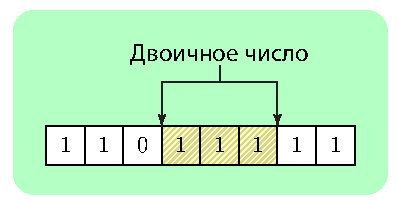
\includegraphics [scale=1] {HML_BinaryToDecimalFromPart_Sheme}
  \caption{Часть бинарной строки} 
  \label{img:HML_BinaryToDecimalFromPart_Sheme}  
\end{figure}

Бинарная подстрока не представляет собой двоичный код целого числа, а представляет код Грея. Его отличительной особенностью является то, что если два целых числа отличаются на единицу, то их коды Грея также будут отличаться только одним битом. Двоичный код не обладает данным свойством.

Существует метод по переводу кода Грея в двоичный код: старший разряд (крайний левый бит) записывается без изменения, каждый следующий символ кода Грея нужно инвертировать, если в двоичном коде перед этим была получена «1», и оставить без изменения, если в двоичном коде был получен «0».
 
 \textbf{Примечание:}
 
 Для перевода всей строки кода Грея в бинарную лучше воспользоваться функцией HML\_GrayCodeToBinary.

 \textbf{Примечание:}

 Для перевода полученной бинарной строки в десятичное число воспользуйтесь функцией HML\_BinaryToDecimal или HML\_BinaryToDecimalFromPart.

 \textbf{Примечание:}
 
 Данная функция используется, например, если в строке Грей кода закодировано несколько десятичных чисел, каждое из которых закодировано своей подстрокой, а общая строка получена склейкой этих строк Грей кода. Для того, чтобы получить десятичные числа проще вначале перевести Грей код в бинарный, а потом бинарный код перевести в десятичный.